\input ../SlidePreamble
\input ../preamble


\begin{document}

{\Huge

  \centerline{\bf TTIC 31230, Fundamentals of Deep Learning}
  \bigskip
  \centerline{David McAllester, Winter 2019}
  \vfill
  \centerline{\bf Discrimination and Constrastive Estimation}
  \vfill
  \centerline{\bf Generative Adversarial Networks (GANs)}
  \vfill
\vfill
\vfill

\slide{Modeling Distributions: Discrimination}

Consider a friendly negative sampling distribution $Q$.

\vfill
Draw $i$ from the uniform distribution on $\{-1,1\}$.

\vfill
For $i = 1$ draw $y$ from $\pop$ and otherwise draw $y$ from $Q$.

\vfill
I will write this as {\color{red} $(i,y) \sim (\pop \uplus Q)$}.

\vfill
{\color{red} $$\Phi^* = \argmin_\Phi E_{(i,y) \sim (\pop \uplus Q)}\;-\ln D_\Phi(i|y)$$}

\slide{Discrimination}

{\color{red} $$\Phi^* = \argmin_\Phi E_{(i,y) \sim (\pop \uplus Q)}\;-\ln D_\Phi(i|y)$$}

Assuming Universality
$$D_{\Phi^*}(1|y) = P(1|y) = \frac{P(1\;\mathrm{and}\; y)}{P(y)} = \frac{\frac{1}{2}\mathrm{Pop}(y)}{\frac{1}{2}\mathrm{Pop}(y) + \frac{1}{2}Q(y)}$$

\vfill
\vfill
{\color{red} $$ \pop(y) = \frac{D_{\Phi^*}(1|y)Q(y)}{1-D_{\Phi^*}(1|y)}$$}

\slide{Descrimination}

The discrimination estimate of $\pop$ is poor when the discrimination problem is easy --- when the discrimination loss can be driven close to zero.

\slide{Modeling Distributions: Contrastive Estimation}

Consider a friendly negative sampling distribution $Q$.

\vfill
Draw one ``positive'' from $\pop$ and $k$ ``negatives'' from $Q$.

\vfill
Shuffle the drawn values into a sequence $y_1,\ldots,y_{k+1}$.

\vfill
Let $i$ be the index of the positive example $y_i$.

\vfill
I will write this as $(i,y_1,\ldots,y_{k+1}) \sim (\pop \uplus Q^k)$.

{\color{red} $$\Phi^* = \argmin_\Phi\; E_{(i,y_1,\ldots,y_{k+1})\sim (\pop\uplus Q^k)} \;- \ln D_\Phi(i|y_1,\ldots,y_{k+1})$$}

\slide{Constrastive Estimation}
{\huge
\begin{eqnarray*}
{\color{red} P(i \;\mathrm{and}\;y_1,\ldots,y_{k+1})} & = & \frac{1}{k+1}\;\pop(y_i)\prod_{j \not = i}Q(y_j) \\
\\
& = & {\color{red} \alpha \frac{\pop(y_i)}{Q(y_i)}},\;\;\;\alpha = \frac{1}{k+1} \prod_i Q(y_i) \\
\\
\\
{\color{red} P(i|y_1,\ldots,y_k)} & = & \frac{P(i\;\mathrm{and}\;y_1,\ldots,y_{k+1})}{\sum_i\; P(i\;\mathrm{and}\;y_1,\ldots,y_{k+1})} \\
\\
\\
& = & {\color{red}  \frac{1}{Z}\;\;\frac{\pop(y_i)}{Q(y_i)}\;\;\;Z = \sum_i \frac{\pop(y_i)}{Q(y_i)}}
\end{eqnarray*}
}

\slide{Constrastive Estimation}

{\color{red} $$\Phi^* = \argmin_\Phi E_{(i,y_1,\ldots,y_{k+1}) \sim (\pop\uplus Q^k)} \;- \ln D_\Phi(i|y_1,\ldots,y_{k+1})$$}
{\color{red} $$D_\Phi(i|y_1,\ldots,y_{k+1}) \doteq \softmax_i s_\Phi(y_i)$$}
{\color{red} $$P(i|y_1,\ldots,y_k) \propto \frac{\pop(y_i)}{Q(y_i)}$$}

Assuming universality:
\begin{eqnarray*}
s_{\Phi^*}(y) & = & \ln \frac{\pop(y)}{Q(y)} + C \;\;\;\mbox{for arbitrary $C$}\\
\\
{\color{red} \pop(y)} & {\color{red} =} & {\color{red} \softmax_y\;\;\; s_{\Phi^*}(y) - \ln Q(y)}
\end{eqnarray*}

\slide{Constrastive Estimation}

The contrastor estimate of $\pop$ is poor when the contrastive problem is easy --- when the contrastive loss can be driven near zero.

\slide{GANs, Goodfellow et al., 2014 (also Schmidhuber 1992)}

Discriminator GAN:
{\color{red} $$\Phi^* = \argmax_\Phi \min_\Psi \;E_{(i,y) \sim (\pop \uplus P_\Phi)} - \ln D_\Psi(i|y)$$}

\vfill
Contrastive GAN:
{\color{red} $$\Phi^* = \argmax_\Phi \min_\Psi \;E_{(i,y_1,\ldots,y_{k+1}) \sim (\pop \uplus P_\Phi^k)} - \ln D_\Psi(i|y_1,\ldots,y_{k+1})$$}

\vfill
Assuming Universality:
{\color{red} $$P_{\Phi^*} = \pop$$}

\slide{Sampling}
\centerline{$z\sim {\cal N}(0,I)$ \hspace{7em} $y\sim P_\Phi$}
\centerline{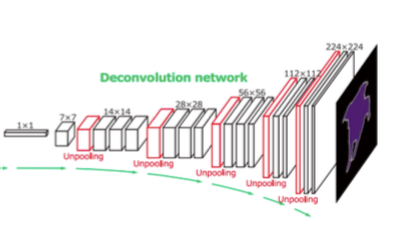
\includegraphics[width=6in]{../images/halfdeconv}}

\slide{Generated Bedrooms(DC GANS, Radford et al., ICLR 2016)}

\centerline{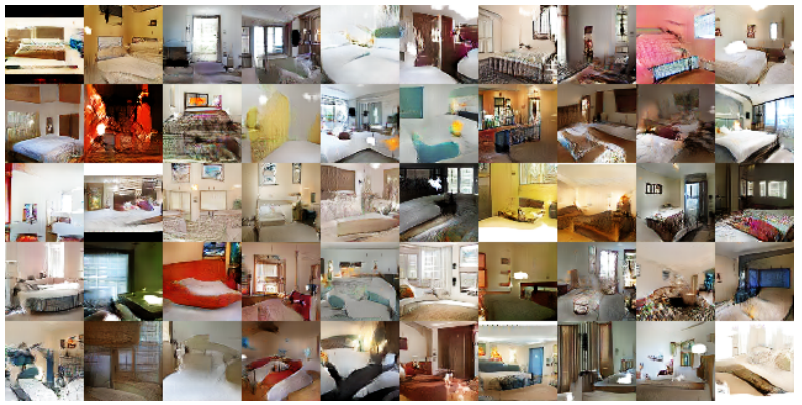
\includegraphics[width = 10in]{../images/Bedrooms}}

\slide{Interpolated Faces}

[Ayan Chakrabarti]

\centerline{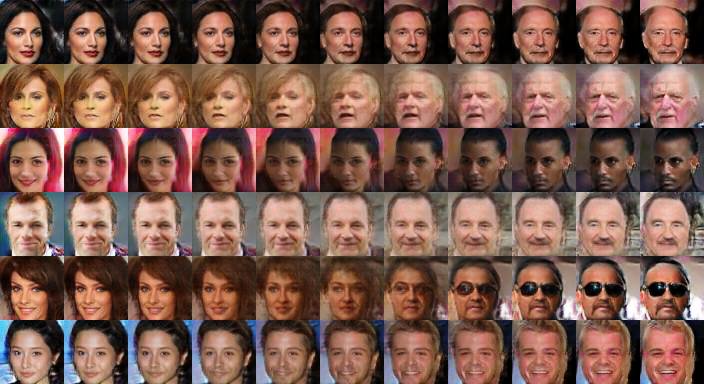
\includegraphics[width = 9in]{../images/interp}}

\slideplain{Image Arithmetic (DC GANS, Radford et al., ICLR 2016)}

\centerline{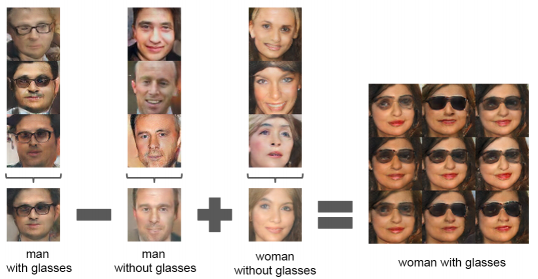
\includegraphics[width = 9in]{../images/ImageFeatures}}

\slide{GANs on Imagenet}

\centerline{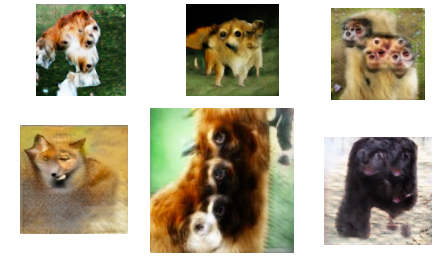
\includegraphics[width = 9in]{../images/BadGAN}}


\slide{Conditional GANs}

All distribution modeling methods apply to conditional distributions.

$${\color{red} \Phi^* = \argmax_\Phi \; \min_\Psi \;\expectsub{(x,y,s) \sim (\mathrm{Pop}\; \uplus \;\mathrm{Pop}(x)P_\Phi(y|x))}
  {-\log P_\Psi(s|x,y)}}$$

\slide{Image-to-Image Translation (Isola et al., 2016)}

\centerline{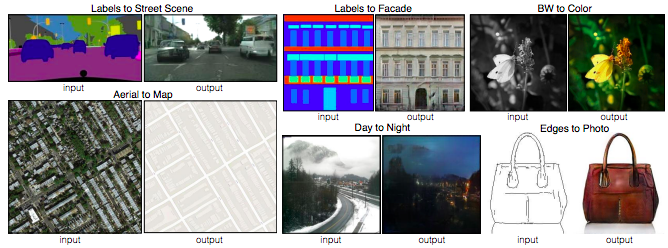
\includegraphics[width = 8.0in]{../images/cGAN0}}

\slide{U-Nets (Ronnenberger et al. 2015)}

\centerline{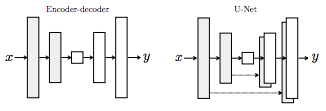
\includegraphics[width = 8.0in]{../images/Unet}}

\slide{Image-to-Image Translation (Isola et al., 2016)}

\centerline{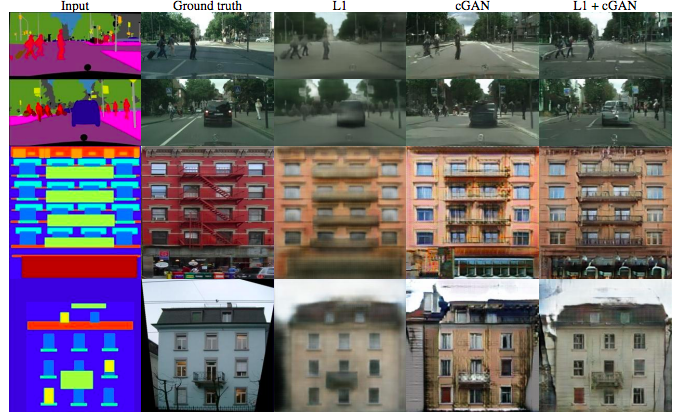
\includegraphics[width = 8.0in]{../images/cGAN1}}

\slide{Arial Photo to Map and Back}

\centerline{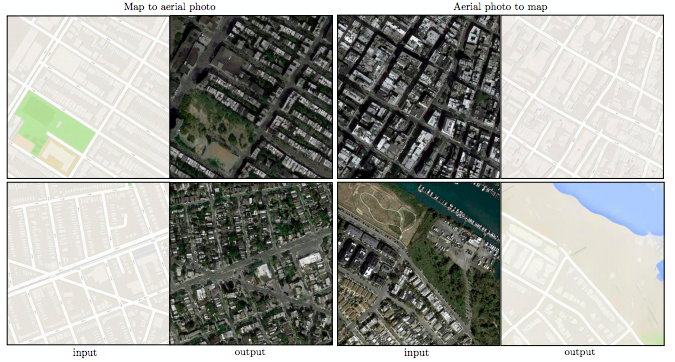
\includegraphics[width = 8.0in]{../images/cGAN2}}

\slide{Colorization}

\centerline{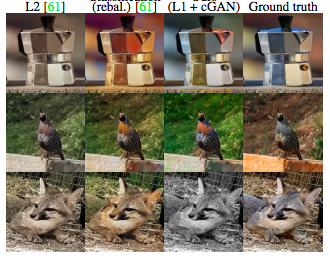
\includegraphics[width = 6.0in]{../images/cGAN3}}

\slide{Semantic Segmentation}

\centerline{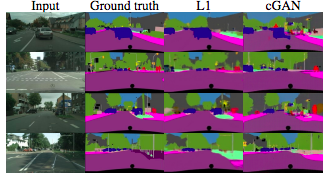
\includegraphics[width = 8.0in]{../images/cGAN4}}

\slide{Cycle Gans (Zhu et al., 2017)}

\centerline{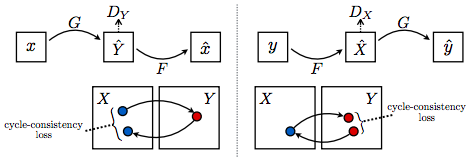
\includegraphics[width = 8.0in]{../images/Cycle2}}


\slide{Cycle Gans}

\centerline{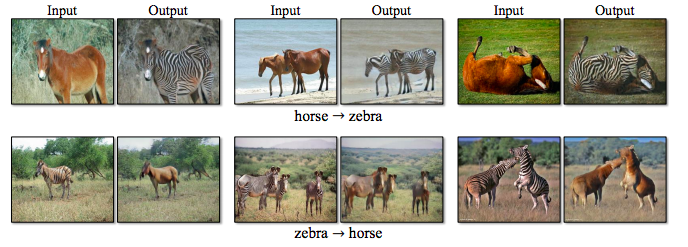
\includegraphics[width = 11.0in]{../images/Cycle3}}

\slide{Cycle Gans}

\centerline{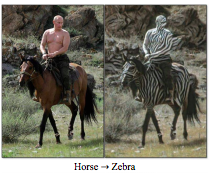
\includegraphics[width = 6.0in]{../images/Cycle4}}

\slidetwo{Cycle Training of Machine Translation}
         {Lample et al, 2017, also Artetxe et al., 2017}

\centerline{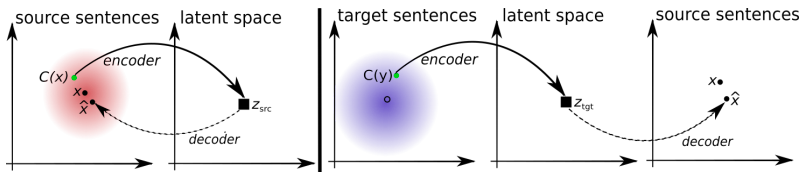
\includegraphics[width = 10.0in]{../images/Cycle5}}

\slide{Text to Speech (Saito et al. 2017)}

\centerline{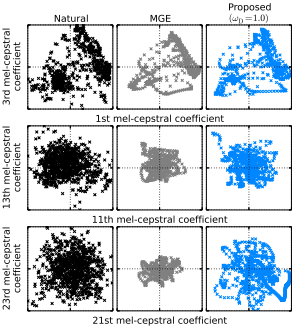
\includegraphics[width = 3.0in]{../images/Txt2spchGAN}}

\vfill
Minimum Generation Error (MGE) uses {\color{red} perceptual distortion} ---
a distance between the feature vector of the generated sound wave and the
feature vector of the original.

\vfill
{\color{red}Perceptual Naturalness} can be enforced by a discriminator.

\slideplain{Adversarial Domain Adaptation (Tzeng et al. 2017)}

\centerline{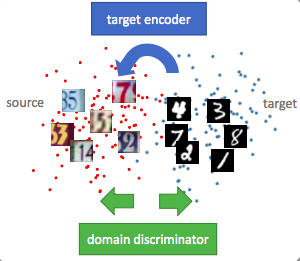
\includegraphics[width = 5.0in]{../images/AdvDomainAdapt}}

\slide{Issues}

\centerline{Jensen-Shannon Divergence}

\vfill
\centerline{Vanishing Gradients}

\vfill
\centerline{Unstable Training}

\vfill
\centerline{Mode Collapse}

\vfill
\centerline{Measuring Perfomance}



\slide{Discrimination: Jensen-Shannon Divergence}

Assuming Universality:
\begin{eqnarray*}
& & {\color{red} E_{(i,y) \sim (\pop\uplus Q)}\;-\ln D_{\Phi^*}(i|y)} \\
\\
& = & E_{(i,y) \sim (\pop\uplus Q)}\;-\ln P(i|y) \\
\\
& = & \frac{1}{2}E_{y \sim \pop} -\ln\;\frac{\pop(y)}{\pop(y) + Q(y)}+ \frac{1}{2} E_{y \sim Q}\; -\ln\;\frac{Q(y)}{\pop(y) + Q(y)} \\
\\
\\
& = & {\color{red} (\ln 2) - \frac{1}{2} \left(\;KL\left(\pop,\frac{\pop+Q}{2}\right),\;KL\left(Q,\frac{\pop+Q}{2}\right)\right)}
\end{eqnarray*}

\slide{Discrimination: Jensen-Shannon Divergence}

\begin{eqnarray*}
& & {\color{red} E_{(i,y) \sim (\pop\uplus Q)}\;-\ln D_{\Phi^*}(i|y)} \\
\\
& = & (\ln 2) - \frac{1}{2} \left(\;KL\left(\pop,\frac{\pop+Q}{2}\right),\;KL\left(Q,\frac{\pop+Q}{2}\right)\right) \\
\\
& = & {\color{red} (\ln 2) - JSD(\pop,Q)}
\end{eqnarray*}

{\color{red} $$0 \leq JSD(P,Q) \leq \ln 2$$}

\slide{Vanishing Gradients}

The discriminator typically ``wins''.

\vfill
The log loss goes to zero (becomes exponentially small) and there is no gradient to guide the generator.

\vfill
In this case the learning stops and the generator is blocked from minimizing $\mathrm{JSD}(\mathrm{Pop},P_\Phi)$.

\slide{A Heuristic Fix}

We continue to use

$$\Psi^*(\Phi) = \argmin_\Psi \;\expectsub{(y,s) \sim (\mathrm{Pop}\; \uplus \;P_\Phi)}{- \log P_\Psi(s|y)}$$

\vfill
But switch the optimization for $\Phi$ from
$$\Phi^* = \argmax_\Phi E_{y \sim P_\Phi}\; - \log P_\Psi(-1|y)$$

to
$$\Phi^* = \argmin_\Phi E_{y \sim P_\Phi}\;- \log P_\Psi(1|y)$$

\vfill
It can be shown that $- \log P_\Psi(1|y)$ is essentially the margin of the binary classifier $\Psi$.

\slide{Converting to Cross Entropy (Goodfellow)}

$$\Psi^*(\Phi) = \argmin_\Psi \;\expectsub{(y,s) \sim (\mathrm{Pop}\; \uplus \;P_\Phi)}{- \log P_\Psi(s|y)}$$

\vfill
$$\mbox{Assume:}\;\;\; P_{\Psi^*}(1|y) = \frac{\mathrm{Pop}(y)}{\mathrm{Pop}(y) + P_\Phi(y)}$$

\vfill
\begin{eqnarray*}
  \mbox{Define:}\;\;\; f_{\Psi^*}(y) & \doteq & \frac{P_{\Psi^*}(1|y)}{P_{\Psi^*}(-1|y)} \\
\\
& = & \frac{\mathrm{Pop}(y)}{P_\Phi(y)}
\end{eqnarray*}

\slide{Converting to Cross Entropy}

\begin{eqnarray*}
 \nabla_\Phi \; E_{y \sim P_\Phi}\;  f_\Psi(y)  & = & \nabla _\Phi \sum_y\; P_\Phi(y) f_\Psi(y) \\
  \\
  & = & \sum_y \; P_\Phi(y) f_\Psi(y) \nabla_\Phi \ln P_\Phi(y) \\
  \\
  & = & \sum_y \;\mathrm{Pop}(y) \nabla_\Phi \ln P_\Phi(y) \\
  \\
  & = & E_{y \sim \mathrm{Pop}} \; \nabla_\Phi \ln P_\Phi(y) \\
  \\
  & = & \nabla_\Phi \; E_{y \sim \mathrm{Pop}} \;\ln P_\Phi(y)
\end{eqnarray*}

\slide{Unstable Training}

Simultaneous gradient descent is not the same as nested max-min.

\vfill
$$\max_\Phi \min_\Psi \;\expectsub{(y,s) \sim (\mathrm{Pop}\; \uplus \;P_\Phi)}{- \log P_\Psi(s|y)}$$

\vfill
vs.

\vfill
$$\min_\Psi \max_\Phi \;\expectsub{(y,s) \sim (\mathrm{Pop}\; \uplus \;P_\Phi)}{- \log P_\Psi(s|y)}$$

\slide{A Synthetic Example}

\centerline{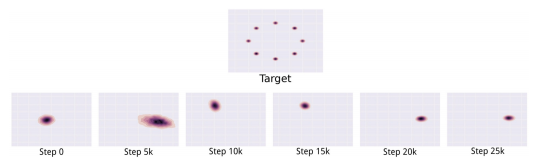
\includegraphics[width=9in]{../images/Unstable1}}

\slide{Another Example}

$${\color{red} \min_x \; \max_y xy}$$

\vfill
A Nash equilibrium is $x= y = 0$.

\vfill
Simultaneous gradient flow yields a circle.

\slide{Mode Collapse a.k.a Mode Dropping}

The generator distribution drops portions of the population.

\centerline{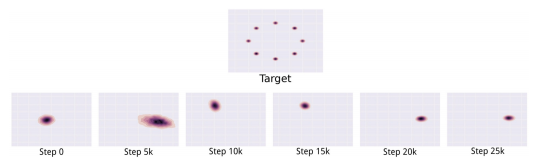
\includegraphics[width=9in]{../images/Unstable1}}

\slide{Measuring Performance}

Most evaluation of GANs is based on subjective judgments of naturalness.

\vfill
This is in contrast to language modeling where performance is directly measured by cross-entropy (bits per character or perplexity).

\slide{Summary}

GANs have not generally proved useful in discriminative tasks such as image segmentation, speech recognition, or machine translation.

\vfill
I predict that there will ultimately be better ways to model distributions (as in language modeling).

\vfill
I predict that in a few years discriminators will be limited to enforcing perceptual naturalness in applications such as
text to speech and image decompression.

\slide{END}

}
\end{document}
